% Section 3: Numerical study. Source: workshop results (oed_multiseed_full_autodiff_results), remat study (src/remat/README.md).
\section{Numerical study}\label{sec:numerical}
\begin{notes}
\item 2-D acoustic, 30 receivers, 10 seeds, fixed sensor count; improvement of the final model MSE over the fixed layout: oracle 18.6\,\%, illumination 16.7\,\%, waveform misfit 9.4\,\%, each in 10/10 seeds (F2). Illumination close to the oracle without true model or extra data: the objective taken to the lab.
\item Example run (F2b): true model, fixed-layout and designed reconstructions, receiver paths (MSE 3449 / 3024 / 3040 / 2668).
\item Cost figure and CPU/GPU benchmark dropped (25 Nov, user): the NeurIPS implementation did not use rematerialisation, so the comparison is not a result of this paper. Rematerialisation is described briefly in Sec.~\ref{sec:method}.
\item Reviewer points (NeurIPS) to address here: $\beta$ sweep, variance over seeds, scaling (answered by the lab plate: 620$\times$520 grid, real data).
\end{notes}
\begin{figure}[ht]\centering
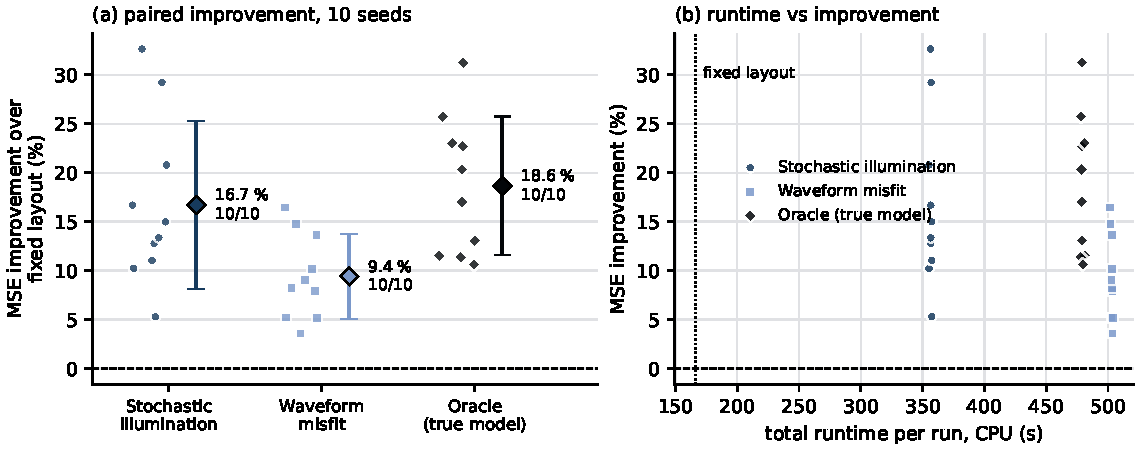
\includegraphics[width=\linewidth]{F2_numerical.pdf}\\[2mm]
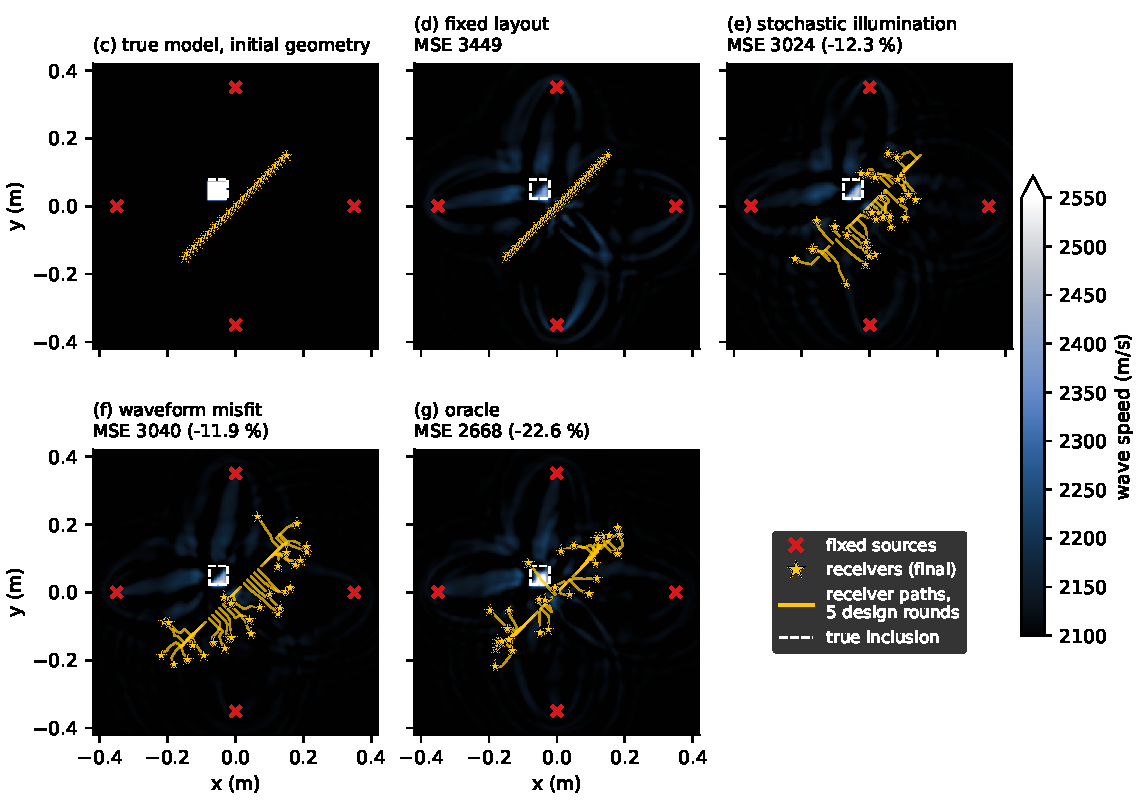
\includegraphics[width=0.85\linewidth]{F2b_numerical_maps.pdf}
\caption{\textbf{Numerical study} (2-D acoustic, 30 receivers, 10 seeds). (a) Paired improvement of the final model MSE over the fixed layout (illumination 16.7\,\%, waveform misfit 9.4\,\%, oracle 18.6\,\%, each 10/10); (b) the same against the total CPU runtime per run. (c--g) Example run: (c) true model with the fixed sources and the initial receiver line; (d) fixed-layout reconstruction; (e--g) reconstructions after 5 design rounds with the receiver paths, for illumination, waveform misfit and the oracle; MSE change relative to (d).}\label{fig:numerical}
\end{figure}

